% ============================================================================
\section{Fault Tolerance and Reconfiguration}
\label{sec:fault_reconfiguration}
% ============================================================================

SPB modularity provides structural redundancy because the converter and
machine are divided into repeated converter--winding modules. However,
fault tolerance is not automatic: because the dc ports are connected
in series, a failed cell can disturb or interrupt the complete dc
current path, a structural challenge demonstrated for SPB and for
other series-connected modular converters alike
\cite{Nikouie2016Fault,Zhang2014FaultToleranceFSCW,Gjerde2014SeriesFault}.
Early SPB work demonstrated post-fault operation under semiconductor
faults, establishing that repeated hardware must
be accompanied by appropriate safe states and control action
\cite{Nikouie2016Fault}. At the
machine level, a submodule short-circuit fault in a modular converter
feeding fractional-slot concentrated-winding PM machines was shown to
drive a fault current above rated current because of the strong
NdFeB rotor magnetization, risking machine overheating; reducing rotor
magnetization limits this fault current but also narrows the
constant-power-speed range, a design tradeoff specific to
fault-tolerant FSCW PM machines \cite{Zhang2014FaultToleranceFSCW}.
In the SPB machine designs of that study, post-fault short-circuit
current with NdFeB magnets exceeds the healthy-phase current, whereas
with ferrite magnets it stays below it, at the cost of becoming
visibly non-sinusoidal from magnetic coupling with the adjacent
healthy windings -- a concrete illustration that PM material selection
is itself a fault-tolerance design variable, not only a torque-density
one. Fault handling in other series-connected modular converters
further underscores that mitigation requires the control system to be
explicitly designed for module isolation \cite{Gjerde2014SeriesFault}.

The machine provides a second layer of redundancy. Healthy winding
groups can potentially redistribute current after phase or converter
faults, as demonstrated in recent multiphase and modular-drive studies
\cite{Tang2025SixPhaseFault,Zhang2025FaultTolerantMMD,
Du2026ModularPMSMFault}. In SPB, however, this machine-side redundancy
is useful only if the failed converter cell can be isolated or bypassed
without breaking the series dc path.

Building on the online reconfiguration capability introduced in
Section~\ref{sec:evolution} \cite{Verkroost2024Reconfiguration}, after
a faulted module is isolated the remaining active set $\mathcal{A}$
must satisfy
\begin{equation}
P^\star=\sum_{k\in\mathcal{A}}P_k^\star,
\label{eq:fault_power_redistribution}
\end{equation}
with torque derating if current, voltage, or thermal limits prevent full
redistribution. Reconfiguration can therefore provide both fault
isolation and an operating-range degree of freedom because the number
of active cells changes the voltage available to the remaining winding
groups. Isolating a cell also raises the voltage that each surviving
cell must share of the fixed dc-link voltage $V_{\mathrm{dc}}$
(\eqref{eq:spb_voltage_sum}, now divided among $|\mathcal{A}|<N$
active cells), which is an additional reason current or power
derating in \eqref{eq:fault_power_redistribution} may be needed after
a fault, as illustrated in Fig.~\ref{fig:spb_fault_response}.
Fig.~\ref{fig:spb_fault_locations} maps these fault locations
onto the SPB structure.

\begin{figure}[!t]
\centering
\begin{tikzpicture}[font=\scriptsize,>=latex,node distance=5mm]
\tikzstyle{cell}=[draw=blue!65!black,rounded corners,minimum width=18mm,
  minimum height=9mm,align=center,fill=blue!8]
\tikzstyle{wind}=[draw=orange!75!black,rounded corners,minimum width=17mm,
  minimum height=7mm,align=center,fill=orange!12,font=\tiny]

\node[cell] (c1) {\textbf{Cell 1}\\[1pt]
  {\tiny SW\textcolor{teal!55!black}{\textcircled{1}} \;\;
  $C_1$\textcolor{teal!55!black}{\textcircled{4}}}};
\node[cell,below=6mm of c1] (c2) {\textbf{Cell 2}\\[1pt]
  {\tiny SW \;\; $C_2$}};
\node[font=\scriptsize,below=2mm of c2] (dots) {$\vdots$};

\node[wind,right=10mm of c1] (w1) {Winding\\group 1};
\node[wind,right=10mm of c2] (w2) {Winding\\group 2};

\draw[->] (c1.east) -- (w1.west)
  node[midway,above,font=\tiny]{\textcolor{teal!55!black}{\textcircled{3}}};
\draw[->] (c2.east) -- (w2.west);

\coordinate (topdc) at ([yshift=4mm]c1.north);
\draw[thick] (topdc) -- (c1.north);
\node[font=\tiny,left] at (topdc) {$+$};
\draw[thick] (c1.south) -- (c2.north)
  node[midway,right,font=\tiny,align=left]{bypass /\\isolation%
  \textcolor{teal!55!black}{\textcircled{2}}};
\draw[thick] (c2.south) -- (dots.north);
\coordinate (botdc) at ([yshift=-4mm]dots.south);
\draw[thick] (dots.south) -- (botdc);
\node[font=\tiny,left] at (botdc) {$-$};

\draw[<->,dashed] ([xshift=-3mm]c1.west) -- ([xshift=-3mm]c2.west)
  node[midway,left,font=\tiny,align=right]{comms\\%
  \textcolor{teal!55!black}{\textcircled{5}}};
\end{tikzpicture}
\caption{Simplified SPB converter--machine structure with fault
locations \textcircled{1}--\textcircled{5} annotated, corresponding in
order to the rows of Table~\ref{tab:spb_fault_compact}.}
\label{fig:spb_fault_locations}
\end{figure}

\begin{table}[!t]
\centering
\caption{SPB Fault Locations and Required System Response}
\label{tab:spb_fault_compact}
\renewcommand{\arraystretch}{1.06}
\setlength{\tabcolsep}{3pt}
\begin{tabular}{p{2.25cm}p{2.7cm}p{2.7cm}}
\hline
\textbf{Fault} & \textbf{SPB consequence} & \textbf{Required response}\\
\hline
Switch / bridge leg & Cell cannot synthesize commanded voltage & Fast safe state and protection \cite{Nikouie2016Fault}\\
Converter module & Series dc path can be interrupted & Bypass/isolation and power redistribution \cite{Verkroost2024Reconfiguration}\\
Winding / phase & Reduced and asymmetric torque capability & Multiphase post-fault current control \cite{Tang2025SixPhaseFault,Du2026ModularPMSMFault}\\
Capacitor / sensor$^{*}$ & Loss of voltage-sharing information or margin & Detection, derating, isolation or shutdown\\
Communication / controller & Loss of distributed coordination & Local fallback and deterministic safe state \cite{Ebrahimian2025FaultTolerantIMMD}\\
\hline
\end{tabular}

\vspace{1mm}
\begin{minipage}{0.95\columnwidth}
\footnotesize
$^{*}$No SPB-specific study directly reports capacitor or sensor fault
handling; this row reflects the authors' system-level inference from
the general modular-converter requirement to detect loss of
cell-voltage sensing or local dc-link capacitance and to derate or
isolate the affected cell accordingly.
\end{minipage}

\end{table}

\begin{figure}[!t]
\centering
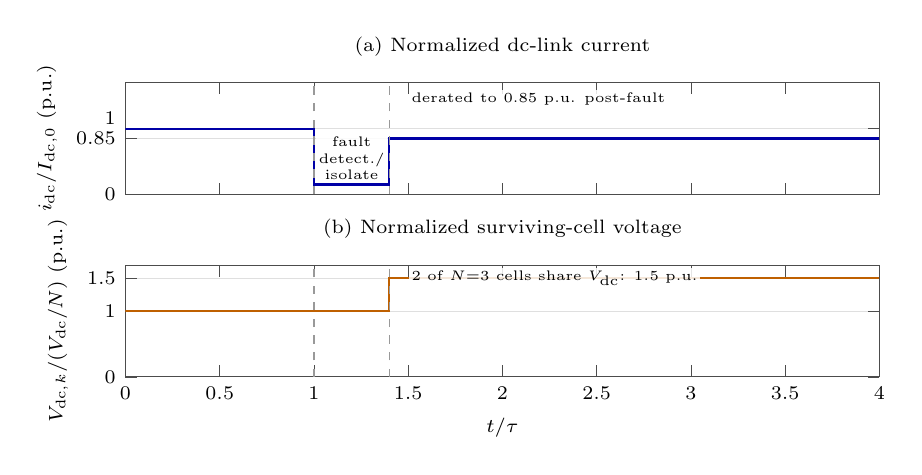
\begin{tikzpicture}
\begin{axis}[
  name=axtop,
  width=0.92\linewidth, height=3.0cm,
  xmin=0,xmax=4, ymin=0,ymax=1.7,
  ylabel={$i_{\mathrm{dc}}/I_{\mathrm{dc},0}$ (p.u.)},
  title={(a) Normalized dc-link current},
  title style={font=\scriptsize}, label style={font=\scriptsize},
  tick label style={font=\scriptsize},
  ymajorgrids, grid style={gray!25},
  xticklabels=\empty,
  ytick={0,0.85},
  extra y ticks={1},
  extra y tick labels={1},
  extra y tick style={tick label style={yshift=1.3mm}},
  axis line style={black!70}, tick style={black!70},
]
\addplot[blue!65!black,thick] coordinates
  {(0,1)(1,1)(1,0.15)(1.4,0.15)(1.4,0.85)(4,0.85)};
\node[font=\tiny,anchor=north west,fill=white,fill opacity=0.85,
  text opacity=1,inner sep=1pt] at (axis cs:1.5,1.6)
  {derated to 0.85~p.u. post-fault};
\draw[dashed,black!40,thin] (axis cs:1,0) -- (axis cs:1,1.7);
\draw[dashed,black!40,thin] (axis cs:1.4,0) -- (axis cs:1.4,1.7);
\node[font=\tiny,align=center,fill=white,fill opacity=0.85,
  text opacity=1,inner sep=1pt] at (axis cs:1.2,0.55)
  {fault\\detect./\\isolate};
\end{axis}
\begin{axis}[
  at={(axtop.south west)}, anchor=north west, yshift=-9mm,
  width=0.92\linewidth, height=3.0cm,
  xmin=0,xmax=4, ymin=0,ymax=1.7,
  xlabel={$t/\tau$}, ylabel={$V_{\mathrm{dc},k}/(V_{\mathrm{dc}}/N)$ (p.u.)},
  title={(b) Normalized surviving-cell voltage},
  title style={font=\scriptsize}, label style={font=\scriptsize},
  tick label style={font=\scriptsize},
  ymajorgrids, grid style={gray!25},
  ytick={0,1,1.5},
  axis line style={black!70}, tick style={black!70},
]
\addplot[orange!75!black,thick] coordinates
  {(0,1)(1.4,1)(1.4,1.5)(4,1.5)};
\node[font=\tiny,anchor=north west,fill=white,fill opacity=0.85,
  text opacity=1,inner sep=1pt] at (axis cs:1.5,1.66)
  {2 of $N{=}3$ cells share $V_{\mathrm{dc}}$: $1.5$~p.u.};
\draw[dashed,black!40,thin] (axis cs:1,0) -- (axis cs:1,1.7);
\draw[dashed,black!40,thin] (axis cs:1.4,0) -- (axis cs:1.4,1.7);
\end{axis}
\end{tikzpicture}
\caption{Illustrative, analytically derived example of the post-fault
current derating and remaining-cell voltage step-up for a
representative $N=3\to2$ case (one of three cells isolated after a
fault); this is not measured or simulated data. (a) Normalized
dc-link current, derated post-fault per
\eqref{eq:fault_power_redistribution}. (b) Normalized remaining-cell
voltage, stepping from 1~p.u. to $N/(N-1)=1.5$~p.u.
\eqref{eq:spb_voltage_sum} once two cells must share $V_{\mathrm{dc}}$.
Both panels share the same time axis.}
\label{fig:spb_fault_response}
\end{figure}

Reliability remains ambiguous because increasing cell count provides
more potential degraded states but also more components that can
fail. System or mission reliability is therefore
more meaningful than component count alone. Markov-chain analysis has
been applied to related fault-tolerant IMMDs to distinguish healthy,
degraded, and failed states \cite{Swanke2022MarkovReliability}, while
integrated distributed traction drives provide additional evidence that
fault tolerance must include both the machine and the local converter
architecture \cite{Hennen2012DistributedIMMD,Wolmarans2008IntegratedFT}.

The direct SPB literature therefore demonstrates the feasibility of
post-fault operation and online reconfiguration, but not yet
automotive-level fault coverage. Detection and isolation time,
short-circuit energy, capacitor and sensor faults, communication loss,
post-fault thermal loading, diagnostic coverage, and deterministic
functional-safety transitions remain important validation topics.
